\documentclass[11pt,a4paper,twoside,french,svgnames]{report}
\usepackage[utf8]{inputenc}
\usepackage[T1]{fontenc}
\usepackage{babel}
% pour compiler avec xelatex
%\usepackage{fontspec,xltxtra,xunicode}

% format de la page
\usepackage[papersize={21cm,29.7cm},margin=1.5cm,bottom=1.5cm%, height=250mm,width=183mm
]{geometry}

% fontes
%\usepackage[upright]{fourier}
\usepackage[boldsans]{ccfonts}
\usepackage{stmaryrd}
\IfFileExists{monster2e.sty}{\usepackage{monster2e}}{} % écrire en très grand
\IfFileExists{bold-extra.sty}{\usepackage{bold-extra}}{}
\IfFileExists{luximono.sty}{\usepackage[scaled=0.9]{luximono}}{}

% graphiques
\usepackage{graphicx}

% références françaises
\usepackage[french]{varioref}

%biblio
\usepackage[nottoc]{tocbibind} % pour que la biblio soit insérée dans la toc
\usepackage[square]{daedale}
\bibliographystyle{cyclope}

% le logo byCC
\usepackage{cclicenses}
\usepackage{cclicence}

%ajoute de l'espace entre le numero de chapitre (chap) et le titre dans la TDM
\usepackage{tocloft}

% Listings INFO 
\usepackage{listings}

\newcommand{\lat}{%
  \lstset{
  language=[AlLaTeX]{TeX},
        escapeinside={(*@}{@*)},
        % numbers=left,
        commentstyle={\sffamily\color{gray}},
        keywordstyle={\large\bfseries\color{black!40!blue}},
        stringstyle={\ttfamily\color{gray}\itshape},
        basicstyle={\ttfamily},
        breaklines=true,
        breakatwhitespace=true,
        showtabs=False,
        showspaces=False,
        showstringspaces=False,
        extendedchars=true,
        emph=[2]{In},
        emphstyle=[2]\color{black!70},
        morecomment=[l][\color{blue}]{Out},
        % aboveskip=1em,
        %belowskip=1em,
        rulecolor=\color{gray},
        backgroundcolor = \color{yellow!20},
        % rulesepcolor=\color{gray},
        %frame=trBL,
        frame=single,
        frameround=tttt,
        framerule=0.3pt,
        framesep=4pt,
        belowcaptionskip=2.1pt,
        title={{\setlength{\fboxsep}{1pt}\fcolorbox{orange}{yellow!20}{\sffamily\scriptsize
              \textcolor{gray!10}{\_}\LaTeX{} \textcolor{gray!10}{\_}}}}}
}


\newcommand{\shell}{%
\lstset{
 language=sh,
        escapeinside={(*@}{@*)},
        %numbers=left,
        commentstyle={\sffamily\color{gray}},
        keywordstyle={\large\bfseries\ttfamily\color{black!70!blue}},
        stringstyle={\ttfamily\color{gray}\itshape},
        basicstyle={\ttfamily},
        breaklines=true,
        breakatwhitespace=true,
        showtabs=False,
        showspaces=False,
        showstringspaces=False,
        extendedchars=true,
        emph=[2]{In},
        emphstyle=[2]\color{black!70},
        morecomment=[l][\color{blue}]{Out},
        %aboveskip=1em,
        %belowskip=1em,
        rulecolor=\color{gray},
        backgroundcolor = \color{blue!10},
        %rulesepcolor=\color{gray},
        %frame=trBL,
        frame=single,
        frameround=tttt,
        framerule=0.3pt,
        framesep=4pt,
        belowcaptionskip=2.1pt,
title={{\setlength{\fboxsep}{1pt}\fcolorbox{blue}{blue!10}{\sffamily\scriptsize
      \textcolor{gray!10}{\_}Shell \textcolor{gray!10}{\_}}}}}
}
% hack pour forcer la compatibilité avec UTF8 (pour le français uniquement)
\lstset{
        extendedchars=true,
        literate={à}{{\`a}}1 {â}{{\^a}}1 %                         lettre a
                 {À}{{\`A}}1 {Â}{{\^A}}1 %                         lettre A
                 {ç}{{\c{c}}}1 %                                   lettre c
                 {Ç}{{\c{C}}}1 %                                   lettre C
                 {é}{{\'e}}1 {è}{{\`e}}1 {ê}{{\^e}}1 {ë}{{\"e}}1 % lettre e
                 {É}{{\'E}}1 {È}{{\`E}}1 {Ê}{{\^E}}1 {Ë}{{\"E}}1 % lettre E
                 {î}{{\^i}}1 {ï}{{\"i}}1 %                         lettre i
                 {Î}{{\^I}}1 {Ï}{{\"I}}1 %                         lettre I
                 {ô}{{\^o}}1 %                                     lettre o
                 {Ô}{{\^O}}1 %                                     lettre O
                 {œ}{{\oe}}1 %                                     lettre oe
                 {Œ}{{\OE}}1 %                                     lettre OE
                 {ù}{{\`u}}1 {û}{{\^u}}1 {ü}{{\"u}}1 %             lettre u
                 {Ù}{{\`U}}1 {Û}{{\^U}}1 {Ü}{{\"U}}1 %             lettre U
}




\usepackage{array}     % Nouveau package de tableau
\usepackage{tabularx}  % Nouveau package de tableau de
                           % fixe largeur
\usepackage{dcolumn}   % alignement sur la virgule
\usepackage{hhline}    % Nouvelle gestion des lignes 
                           % horizontales dans les tableaux
\usepackage{multirow}  % package permettant de d'\'erire sur plusieures
                           % lignes dans un tableau
\usepackage{slashbox}  % ligne diagonale dans une case


\usepackage[detect-all]{siunitx} % unités et format des nombres

\usepackage{xcolor} % les couleurs
\definecolor{ciel}{rgb}{0.220,0.890,0.999}




\setcounter{tocdepth}{3} % profondeur de TDM
\pagenumbering{arabic} % numérotation des pages


%%%%%%%%%%%%%%%%%%%%%%%%%%%%%%%
% %%% Gestion des espaces % %%%
%%%%%%%%%%%%%%%%%%%%%%%%%%%%%%%

\usepackage{xspace}	    % Pour bien g\'eer les espaces \'ela fin de macros 

%%%%%%%%%%%%%%%%%%%%%%%%%%%%%%%%%%
% %%% Gestion conditionnelle % %%%
%%%%%%%%%%%%%%%%%%%%%%%%%%%%%%%%%%


\usepackage{calc}              % permet les calculs
\usepackage{lastpage}   % utilis\'edans tounez la page 
                          



%%%%%%%%%%%%%%%%%%%%%%%%%%%%%%%%%%%
% Entete et pied de page
%%%%%%%%%%%%%%%%%%%%%%%%%%%%%%%%%

\usepackage{fancyhdr}%,fancybox} conflit avec fancyvrb quand on met une option \`a VerbatimOut




% en-tête et pieds de pages reformatés avec fancyhdr
\newcommand{\entet}[3]{
\fancyfoot[C]{{\scriptsize\textsl{  Guillaume  \textsc{Connan} -  Atelier  Linux  Nantes - #3 - \today}}}
 \fancyhead[RO,LE]{\color{MidnightBlue}\fontfamily{ugq}\selectfont\bfseries\thepage} \fancyhead[RE,LO]{ }
 \fancyhead[CO]{\color{black!80}\fontfamily{ugq}\selectfont     #1     }
 \fancyhead[CE]{\color{MidnightBlue}\fontfamily{ugq}\selectfont\MakeLowercase
     #2  }
\renewcommand{\headrulewidth}{0.4pt}
 \pagestyle{fancy}
}

\entet{\leftmark }{\rightmark }{\href{http://informathix.tuxfamily.org/}{Licence
    Creative Commons}\byncsa}%g,d,b


% un nouveau style de théorème
\newtheorem{definition}{D\'efinition}[chapter]
\renewcommand{\thedefinition}{\thechapter\, - \arabic{definition}}


% pour faire de belles figures
\usepackage{tikz}
\usetikzlibrary{automata,fit,trees,matrix,arrows,decorations.pathmorphing,shapes.arrows,chains,positioning,intersections,backgrounds,calc,through,mindmap}
\usepackage{amssymb,amsbsy,amsfonts,amstext,amscd,amsopn,amsxtra}

% liens hypertexte
\usepackage[colorlinks=true,linkcolor=red!50!blue,citecolor=red,pdfauthor={Guillaume CONNAN},bookmarks,pdfpagelabels]{hyperref}


% le chemin vers les graphiques et les images à insérer 
\graphicspath{{/home/moi/VISA_III/figures_visa/}{/home/moi/Lycee/TDmaple/2006_7/}{/home/moi/Figures/Arbres_Graphes/}{/home/moi/Figures/FigSTI/}{/home/moi/Figures/FigMaple/}{/home/moi/Photos/Maths/}{/home/moi/Photos/Tehessin/}{/home/moi/Figures/FigSTI/}{/home/moi/Figures/FigSeconde/}{/home/moi/Lycee/Informatique/XCAS/2008_9/}{/home/moi/Lycee/TDmaple/2008_9/}{/home/moi/IUT/Thierry/Conversions/}{/home/moi/Photos/informathix/}{/home/moi/Lycee/Informatique/PafAlgo/}{/home/moi/Figures/figuresAlice/}{/home/moi/Figures/FigSeconde/}{/home/moi/Biocam/robot/}{/home/moi/Biocam/CoursIni3d/}{/home/moi/Biocam/central/figures/}{/home/moi/Biocam/central/}{/home/moi/IUT/INFO2/Images/}{/home/moi/IUT/INFO2/2011_12/graphes/}{/home/moi/IUT/INFO1/CM1/}{/home/moi/Figures/figuresTS/}{/home/moi/Photos/Tehessin/}{/home/moi/Figures/FigSTI/}{/home/moi/Alice/figures3/}{/home/moi/Alice/figures3/newcourbes/}{/home/moi/Alice/figures/}{/home/moi/Figures/figuresAlice/}{/home/moi/Photos/Maths/}{/home/moi/Lycee/TS/}{/home/moi/Lycee/TS/2009_10/}{/home/moi/Figures/FigMaple/}{/home/moi/Figures/figuresTS/newcourbes/}{/home/moi/Figures/FigEspace/}}




%% INDEX
\usepackage{makeidx,showidx}
\usepackage{index}
\makeindex
\renewindex{default}{idx}{ind}{Un exemple d'index}


%% GLOSSAIRE
\usepackage{glossaries}
\makeglossaries
\loadglsentries{LinuxGlossaire}


% pas d'indentation 
\setlength{\parindent}{0mm}


%%
%% le titre

\title{UN RAPPORT EN \LaTeX{}
\\
\scalebox{0.75}[0.75]{\emph{Pour les débutatnts}}
}
\author{Guillaume \textsc{Connan}\thanks{ Université de
  Nantes}             }


\date{Atelier Linux Nantes - 8 février 2014}

% page de titre 
\makeatletter
\renewcommand{\maketitle}{%
  \begin{titlepage}
  \centering
      {\HUGE \textsc{Université de Nantes}}\\
      \textsc{Institut de Recherhce sur l'Enseignement des Mathématiques}\\
    \vspace{1cm}
      \includegraphics[width=0.25\textwidth]{logo_iut_coul.jpg}
      \hfill
      \includegraphics[width=0.45\textwidth]{logo_uni_bleu}\\
    \vspace{1cm}
      {\huge	\@date}\\
    \vfill
    \par
    \hrulefill
    \par
       {\Huge \@title} \\
    \par
    \hrulefill
    \par
 \vspace{2em}
% Author and supervisor
{
\begin{minipage}{0.4\textwidth}
\begin{flushleft} \LARGE
\emph{Auteur:}\\
Guillaume \textsc{Connan}
\end{flushleft}
\end{minipage}
\begin{minipage}{0.4\textwidth}
\begin{flushright} \LARGE
\emph{Superviseur:} \\
Dr.~Stéphane \textsc{Grognet}
\end{flushright}
\end{minipage}
}
    \vfill
        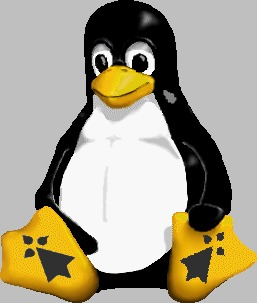
\includegraphics[height=0.2\textheight]{linux_nantes}
        \hfill
        
\includegraphics[height=0.2\textheight]{irem_heron}
  \end{titlepage}
}
\makeatother

%
%
%
% FIΝ DU PRÉAMBULE 
%
%





\begin{document}

% Insertion du titre

\maketitle

% TDM

\tableofcontents

% les chapitres inclus

\renewcommand\chaptername{Atelier \No}
\chapter{Qu'est-ce que \LaTeX{}?}

\section{L'origine}

Pour tout savoir, lisez l'introduction écrite par Vincent \textsc{Lozano} dans son ouvrage
\textit{Tout ce  que vous avez  toujours voulu  savoir sur {\LaTeX}  sans jamais
  oser le demander}\citep{toutLatex} qui est  disponible gratuitement en ligne à
l'adresse
\href{http://www.framabook.org/latex.html}{http://www.framabook.org/latex.html}
ou au format papier pour un prix ridiculement modique. Tout est dit (vous pouvez également écouter le conférencier
pendant l'atelier). Citons en particulier: 

{\itshape
\begin{quote}
Il existe plusieurs raisons pour lesquelles il est \og impératif\fg{} de ne
pas utiliser \LaTeX{}:
\begin{enumerate}
\item vous utilisez un traitement de texte uniquement pour faire vos
  cartes de v\oe{}ux, votre courrier, pour noter quelques idées, etc.
  ;
\item vous adorez les souris (1 ou 3 boutons indifféremment) et vous
  pensez que la seule manière d'écrire des équations est de les
  utiliser (les souris) de manière intensive;
\item vous pensez qu'UNIX c'est « prise de tête » et « pas
  convivial » et/ou vous avez une aversion particulière pour tout
  langage de programmation;
\item vous trouvez normal: \primo que votre logiciel préféré ne
  puisse pas lire le document que vous aviez produit avec la version
  précédente, et/ou \secundo que la nouvelle version vous oblige à
  changer de système d'exploitation, et \tertio que la nouvelle
  version dudit système d'exploitation vous oblige à changer
  d'ordinateur, et \quarto que votre nouvel ordinateur...
\item vous ne savez pas où se trouve la touche \verb+\+ sur 
  votre clavier. \label{nbraisons}
\end{enumerate}
Si vous vous reconnaissez dans une de ces catégories, mieux vaut vous
contenter de votre système actuel.
\end{quote}
}

Un  autre  bon  livre  est  celui de  Denis  \textsc{Bitouzé}  et  de  Jean-Côme
\textsc{Charpentier} \citep{introductionLatex}. Tous deux sont d'ailleurs  venus à
Nantes  en  2006 pour  encadrer  un  stage  \gls{latex} organisé  également  par
l'\textsc{Irem}.

Des membres de l'équipe qui maintiennent  \LaTeX{} ont également mis en ligne la
\textit{Not so short introduction to \LaTeX{}} ou apprendre \LaTeX{} en 166 minutes.

\href{http://hivernal.org/static/computing/doc/lshort-fr.fr.html}{http://hivernal.org/static/computing/doc/lshort-fr.fr.html}


Le livre que j'ai  le plus consulté est le \textit{\LaTeX{}  par la pratique} de
Christian  \textsc{Rolland} \citep{rolland1999}  mais la  \og bible\fg{}  est le
\LaTeX{} Companion \citep{companionfr}.







\section{Principe}

\LaTeX{}  n'est pas  \textsc{Wysiwyg} (pour  \textit{What  You See  Is all  What
  You've Got} comme disait Brian \textsc{Kernighan},  l'un des pères du C...) et
bien heureusement. Cela permet à l'utilisateur(rice) de bien séparer la forme du
fond et surtout de na pas coder \og  en dur\fg{} la mise en forme pour gagner en
portabilité et  en souplesse. Vous  pouvez changer totalement l'aspect  de votre
document sans toucher  au fichier source. C'est le principe  de base d'une 
programmation bien pensée.






\section{Installation}\index{Installation}

Il  suffit  d'installer  la  distribution \TeX{}Live  présente  sur  toutes  les
distributions.  Elle dispose  en  particulier de  \texttt{tlmgr}  qui permet  de
mettre à jour et d'installer facilement de nouvelles extensions:


\shell

\begin{lstlisting}
$ tlmgr update --all
tlmgr: package repository http://mirror.ibcp.fr/pub/CTAN/systems/texlive/tlnet
tlmgr: saving backups to /usr/local/texlive/2013/tlpkg/backups
[  1/256, ??:??/??:??] update: abntex2 [4523k] (31530 -> 32794) ... done
[  2/256, 00:46/45:59] update: achemso [470k] (31893 -> 32619) ... done
...
tlmgr: package log updated: /usr/local/texlive/2013/texmf-var/web2c/tlmgr.log
running mktexlsr ...
running mtxrun --generate ...
running updmap-sys ...
regenerating fmtutil.cnf in /usr/local/texlive/2013/texmf-var
running fmtutil-sys --no-error-if-no-format --byengine ptex ...
running fmtutil-sys --no-error-if-no-format --byengine eptex ...
running fmtutil-sys --no-error-if-no-format --byengine pdftex ...
running fmtutil-sys --byfmt cont-en ...
\end{lstlisting}


Cependant,   certaines   distributions  ne   disposent   pas   de  la   dernière
\TeX{}Live qui est disponible à cette adresse:


\begin{center}
  \href{https://www.tug.org/texlive/}{https://www.tug.org/texlive/}
\end{center}

 Pour y remédier, il ne faut pas passer par les dépôts mais suivre
les instructions disponible sur:

\begin{center}
\href{https://www.tug.org/texlive/quickinstall.html}{https://www.tug.org/texlive/quickinstall.html}
\end{center}

puis  se reporter  sur  l'installation d'un  dépôt  Debian ou  Ubuntu  \og à  la
vanille\fg{}:

\begin{center}
\href{https://www.tug.org/texlive/debian.html}{https://www.tug.org/texlive/debian.html}
\end{center}

pour berner le gestionnaire de paquets sur les \og Debian like\fg{}.


\section{Quel éditeur?}\index{\'{E}diteur}

Il vous  faut un  environnement de  travail. Le  meilleur est  bien sur  le mode
AUC\TeX{} d'emacs.

Vous pouvez utiliser par ailleurs les éditeurs dédiés Kile et \TeX{}maker. 

Gedit dispose d'un greffon dédié. Tout est expliqué par Denis \textsc{Le Fur}:

\begin{center}
  \href{http://mathsp.tuxfamily.org/spip.php?article9}{http://mathsp.tuxfamily.org/spip.php?article9}
\end{center}



Il vous faut ensuite une bonne visionneuse de PDF comme par exemple Zathura.

\section{Quel moteur?}

Écoutez les conseils de votre conférencier.








% Pour               les              thèses,               la              classe
% \href{http://www.loria.fr/~roegel/TeX/TUL.html}{thesUL}.


% Pour créer le glossaire, il faut dans un shell taper:


% \shell
% \begin{lstlisting}
% $ makeglossaries FichierPrincipal
% \end{lstlisting}


% \index{cadratin}, hauteur d'x.





%%% Local Variables: 
%%% TeX-master: "ExempleRapport"
%%% End: 

\chapter{Composer un document}


\section{Le préambule}

Décortiquons le préambule de ce simple rapport.

\lat

La classe, l'encodage:

\begin{lstlisting}
\documentclass[11pt,a4paper,twoside,french,svgnames]{report}
\usepackage[utf8]{inputenc}
\usepackage[T1]{fontenc}
\usepackage{babel}
\end{lstlisting}

Le format de la page:

\begin{lstlisting}
\usepackage[papersize={21cm,29.7cm},margin=1.5cm,bottom=1.5cm]{geometry}
\end{lstlisting}

Les fontes:

\begin{lstlisting}
%\usepackage[upright]{fourier}
%\usepackage{lmodern}
\usepackage[boldsans]{ccfonts}
\usepackage{stmaryrd}
% optionnel : pour avoir de plus belles fontes à chasse fixe et en gras
\IfFileExists{bold-extra.sty}{\usepackage{bold-extra}}{}
\IfFileExists{luximono.sty}{\usepackage[scaled=0.9]{luximono}}{}
\end{lstlisting}


Puis un certain nombre de chargement d'extensions, d'options, de macros (voir le
fichier source principal de ce document \verb+ExempleRapport.tex+).

Enfin le titre:

\begin{lstlisting}
\title{UN RAPPORT EN \LaTeX{} \\
\scalebox{0.75}[0.75]{\emph{Pour les débutatnts}}
}

\author{Guillaume \textsc{Connan}\thanks{ Université de Nantes}}

\date{Atelier Linux Nantes - 8 février 2014}
\end{lstlisting}


\section{Le corps du document}

\begin{lstlisting}
\begin{document}

% Insertion du titre
\maketitle
% TDM
\tableofcontents
% les chapitres inclus
\renewcommand\chaptername{Atelier \No}
\chapter{Qu'est-ce que \LaTeX{}?}

\section{L'origine}

Pour tout savoir, lisez l'introduction écrite par Vincent \textsc{Lozano} dans son ouvrage
\textit{Tout ce  que vous avez  toujours voulu  savoir sur {\LaTeX}  sans jamais
  oser le demander}\citep{toutLatex} qui est  disponible gratuitement en ligne à
l'adresse
\href{http://www.framabook.org/latex.html}{http://www.framabook.org/latex.html}
ou au format papier pour un prix ridiculement modique. Tout est dit (vous pouvez également écouter le conférencier
pendant l'atelier). Citons en particulier: 

{\itshape
\begin{quote}
Il existe plusieurs raisons pour lesquelles il est \og impératif\fg{} de ne
pas utiliser \LaTeX{}:
\begin{enumerate}
\item vous utilisez un traitement de texte uniquement pour faire vos
  cartes de v\oe{}ux, votre courrier, pour noter quelques idées, etc.
  ;
\item vous adorez les souris (1 ou 3 boutons indifféremment) et vous
  pensez que la seule manière d'écrire des équations est de les
  utiliser (les souris) de manière intensive;
\item vous pensez qu'UNIX c'est « prise de tête » et « pas
  convivial » et/ou vous avez une aversion particulière pour tout
  langage de programmation;
\item vous trouvez normal: \primo que votre logiciel préféré ne
  puisse pas lire le document que vous aviez produit avec la version
  précédente, et/ou \secundo que la nouvelle version vous oblige à
  changer de système d'exploitation, et \tertio que la nouvelle
  version dudit système d'exploitation vous oblige à changer
  d'ordinateur, et \quarto que votre nouvel ordinateur...
\item vous ne savez pas où se trouve la touche \verb+\+ sur 
  votre clavier. \label{nbraisons}
\end{enumerate}
Si vous vous reconnaissez dans une de ces catégories, mieux vaut vous
contenter de votre système actuel.
\end{quote}
}

Un  autre  bon  livre  est  celui de  Denis  \textsc{Bitouzé}  et  de  Jean-Côme
\textsc{Charpentier} \citep{introductionLatex}. Tous deux sont d'ailleurs  venus à
Nantes  en  2006 pour  encadrer  un  stage  \gls{latex} organisé  également  par
l'\textsc{Irem}.

Des membres de l'équipe qui maintiennent  \LaTeX{} ont également mis en ligne la
\textit{Not so short introduction to \LaTeX{}} ou apprendre \LaTeX{} en 166 minutes.

\href{http://hivernal.org/static/computing/doc/lshort-fr.fr.html}{http://hivernal.org/static/computing/doc/lshort-fr.fr.html}


Le livre que j'ai  le plus consulté est le \textit{\LaTeX{}  par la pratique} de
Christian  \textsc{Rolland} \citep{rolland1999}  mais la  \og bible\fg{}  est le
\LaTeX{} Companion \citep{companionfr}.







\section{Principe}

\LaTeX{}  n'est pas  \textsc{Wysiwyg} (pour  \textit{What  You See  Is all  What
  You've Got} comme disait Brian \textsc{Kernighan},  l'un des pères du C...) et
bien heureusement. Cela permet à l'utilisateur(rice) de bien séparer la forme du
fond et surtout de na pas coder \og  en dur\fg{} la mise en forme pour gagner en
portabilité et  en souplesse. Vous  pouvez changer totalement l'aspect  de votre
document sans toucher  au fichier source. C'est le principe  de base d'une 
programmation bien pensée.






\section{Installation}\index{Installation}

Il  suffit  d'installer  la  distribution \TeX{}Live  présente  sur  toutes  les
distributions.  Elle dispose  en  particulier de  \texttt{tlmgr}  qui permet  de
mettre à jour et d'installer facilement de nouvelles extensions:


\shell

\begin{lstlisting}
$ tlmgr update --all
tlmgr: package repository http://mirror.ibcp.fr/pub/CTAN/systems/texlive/tlnet
tlmgr: saving backups to /usr/local/texlive/2013/tlpkg/backups
[  1/256, ??:??/??:??] update: abntex2 [4523k] (31530 -> 32794) ... done
[  2/256, 00:46/45:59] update: achemso [470k] (31893 -> 32619) ... done
...
tlmgr: package log updated: /usr/local/texlive/2013/texmf-var/web2c/tlmgr.log
running mktexlsr ...
running mtxrun --generate ...
running updmap-sys ...
regenerating fmtutil.cnf in /usr/local/texlive/2013/texmf-var
running fmtutil-sys --no-error-if-no-format --byengine ptex ...
running fmtutil-sys --no-error-if-no-format --byengine eptex ...
running fmtutil-sys --no-error-if-no-format --byengine pdftex ...
running fmtutil-sys --byfmt cont-en ...
\end{lstlisting}


Cependant,   certaines   distributions  ne   disposent   pas   de  la   dernière
\TeX{}Live qui est disponible à cette adresse:


\begin{center}
  \href{https://www.tug.org/texlive/}{https://www.tug.org/texlive/}
\end{center}

 Pour y remédier, il ne faut pas passer par les dépôts mais suivre
les instructions disponible sur:

\begin{center}
\href{https://www.tug.org/texlive/quickinstall.html}{https://www.tug.org/texlive/quickinstall.html}
\end{center}

puis  se reporter  sur  l'installation d'un  dépôt  Debian ou  Ubuntu  \og à  la
vanille\fg{}:

\begin{center}
\href{https://www.tug.org/texlive/debian.html}{https://www.tug.org/texlive/debian.html}
\end{center}

pour berner le gestionnaire de paquets sur les \og Debian like\fg{}.


\section{Quel éditeur?}\index{\'{E}diteur}

Il vous  faut un  environnement de  travail. Le  meilleur est  bien sur  le mode
AUC\TeX{} d'emacs.

Vous pouvez utiliser par ailleurs les éditeurs dédiés Kile et \TeX{}maker. 

Gedit dispose d'un greffon dédié. Tout est expliqué par Denis \textsc{Le Fur}:

\begin{center}
  \href{http://mathsp.tuxfamily.org/spip.php?article9}{http://mathsp.tuxfamily.org/spip.php?article9}
\end{center}



Il vous faut ensuite une bonne visionneuse de PDF comme par exemple Zathura.

\section{Quel moteur?}

Écoutez les conseils de votre conférencier.








% Pour               les              thèses,               la              classe
% \href{http://www.loria.fr/~roegel/TeX/TUL.html}{thesUL}.


% Pour créer le glossaire, il faut dans un shell taper:


% \shell
% \begin{lstlisting}
% $ makeglossaries FichierPrincipal
% \end{lstlisting}


% \index{cadratin}, hauteur d'x.





%%% Local Variables: 
%%% TeX-master: "ExempleRapport"
%%% End: 

\chapter{Composer un document}


\section{Le préambule}

Décortiquons le préambule de ce simple rapport.

\lat

La classe, l'encodage:

\begin{lstlisting}
\documentclass[11pt,a4paper,twoside,french,svgnames]{report}
\usepackage[utf8]{inputenc}
\usepackage[T1]{fontenc}
\usepackage{babel}
\end{lstlisting}

Le format de la page:

\begin{lstlisting}
\usepackage[papersize={21cm,29.7cm},margin=1.5cm,bottom=1.5cm]{geometry}
\end{lstlisting}

Les fontes:

\begin{lstlisting}
%\usepackage[upright]{fourier}
%\usepackage{lmodern}
\usepackage[boldsans]{ccfonts}
\usepackage{stmaryrd}
% optionnel : pour avoir de plus belles fontes à chasse fixe et en gras
\IfFileExists{bold-extra.sty}{\usepackage{bold-extra}}{}
\IfFileExists{luximono.sty}{\usepackage[scaled=0.9]{luximono}}{}
\end{lstlisting}


Puis un certain nombre de chargement d'extensions, d'options, de macros (voir le
fichier source principal de ce document \verb+ExempleRapport.tex+).

Enfin le titre:

\begin{lstlisting}
\title{UN RAPPORT EN \LaTeX{} \\
\scalebox{0.75}[0.75]{\emph{Pour les débutatnts}}
}

\author{Guillaume \textsc{Connan}\thanks{ Université de Nantes}}

\date{Atelier Linux Nantes - 8 février 2014}
\end{lstlisting}


\section{Le corps du document}

\begin{lstlisting}
\begin{document}

% Insertion du titre
\maketitle
% TDM
\tableofcontents
% les chapitres inclus
\renewcommand\chaptername{Atelier \No}
\chapter{Qu'est-ce que \LaTeX{}?}

\section{L'origine}

Pour tout savoir, lisez l'introduction écrite par Vincent \textsc{Lozano} dans son ouvrage
\textit{Tout ce  que vous avez  toujours voulu  savoir sur {\LaTeX}  sans jamais
  oser le demander}\citep{toutLatex} qui est  disponible gratuitement en ligne à
l'adresse
\href{http://www.framabook.org/latex.html}{http://www.framabook.org/latex.html}
ou au format papier pour un prix ridiculement modique. Tout est dit (vous pouvez également écouter le conférencier
pendant l'atelier). Citons en particulier: 

{\itshape
\begin{quote}
Il existe plusieurs raisons pour lesquelles il est \og impératif\fg{} de ne
pas utiliser \LaTeX{}:
\begin{enumerate}
\item vous utilisez un traitement de texte uniquement pour faire vos
  cartes de v\oe{}ux, votre courrier, pour noter quelques idées, etc.
  ;
\item vous adorez les souris (1 ou 3 boutons indifféremment) et vous
  pensez que la seule manière d'écrire des équations est de les
  utiliser (les souris) de manière intensive;
\item vous pensez qu'UNIX c'est « prise de tête » et « pas
  convivial » et/ou vous avez une aversion particulière pour tout
  langage de programmation;
\item vous trouvez normal: \primo que votre logiciel préféré ne
  puisse pas lire le document que vous aviez produit avec la version
  précédente, et/ou \secundo que la nouvelle version vous oblige à
  changer de système d'exploitation, et \tertio que la nouvelle
  version dudit système d'exploitation vous oblige à changer
  d'ordinateur, et \quarto que votre nouvel ordinateur...
\item vous ne savez pas où se trouve la touche \verb+\+ sur 
  votre clavier. \label{nbraisons}
\end{enumerate}
Si vous vous reconnaissez dans une de ces catégories, mieux vaut vous
contenter de votre système actuel.
\end{quote}
}

Un  autre  bon  livre  est  celui de  Denis  \textsc{Bitouzé}  et  de  Jean-Côme
\textsc{Charpentier} \citep{introductionLatex}. Tous deux sont d'ailleurs  venus à
Nantes  en  2006 pour  encadrer  un  stage  \gls{latex} organisé  également  par
l'\textsc{Irem}.

Des membres de l'équipe qui maintiennent  \LaTeX{} ont également mis en ligne la
\textit{Not so short introduction to \LaTeX{}} ou apprendre \LaTeX{} en 166 minutes.

\href{http://hivernal.org/static/computing/doc/lshort-fr.fr.html}{http://hivernal.org/static/computing/doc/lshort-fr.fr.html}


Le livre que j'ai  le plus consulté est le \textit{\LaTeX{}  par la pratique} de
Christian  \textsc{Rolland} \citep{rolland1999}  mais la  \og bible\fg{}  est le
\LaTeX{} Companion \citep{companionfr}.







\section{Principe}

\LaTeX{}  n'est pas  \textsc{Wysiwyg} (pour  \textit{What  You See  Is all  What
  You've Got} comme disait Brian \textsc{Kernighan},  l'un des pères du C...) et
bien heureusement. Cela permet à l'utilisateur(rice) de bien séparer la forme du
fond et surtout de na pas coder \og  en dur\fg{} la mise en forme pour gagner en
portabilité et  en souplesse. Vous  pouvez changer totalement l'aspect  de votre
document sans toucher  au fichier source. C'est le principe  de base d'une 
programmation bien pensée.






\section{Installation}\index{Installation}

Il  suffit  d'installer  la  distribution \TeX{}Live  présente  sur  toutes  les
distributions.  Elle dispose  en  particulier de  \texttt{tlmgr}  qui permet  de
mettre à jour et d'installer facilement de nouvelles extensions:


\shell

\begin{lstlisting}
$ tlmgr update --all
tlmgr: package repository http://mirror.ibcp.fr/pub/CTAN/systems/texlive/tlnet
tlmgr: saving backups to /usr/local/texlive/2013/tlpkg/backups
[  1/256, ??:??/??:??] update: abntex2 [4523k] (31530 -> 32794) ... done
[  2/256, 00:46/45:59] update: achemso [470k] (31893 -> 32619) ... done
...
tlmgr: package log updated: /usr/local/texlive/2013/texmf-var/web2c/tlmgr.log
running mktexlsr ...
running mtxrun --generate ...
running updmap-sys ...
regenerating fmtutil.cnf in /usr/local/texlive/2013/texmf-var
running fmtutil-sys --no-error-if-no-format --byengine ptex ...
running fmtutil-sys --no-error-if-no-format --byengine eptex ...
running fmtutil-sys --no-error-if-no-format --byengine pdftex ...
running fmtutil-sys --byfmt cont-en ...
\end{lstlisting}


Cependant,   certaines   distributions  ne   disposent   pas   de  la   dernière
\TeX{}Live qui est disponible à cette adresse:


\begin{center}
  \href{https://www.tug.org/texlive/}{https://www.tug.org/texlive/}
\end{center}

 Pour y remédier, il ne faut pas passer par les dépôts mais suivre
les instructions disponible sur:

\begin{center}
\href{https://www.tug.org/texlive/quickinstall.html}{https://www.tug.org/texlive/quickinstall.html}
\end{center}

puis  se reporter  sur  l'installation d'un  dépôt  Debian ou  Ubuntu  \og à  la
vanille\fg{}:

\begin{center}
\href{https://www.tug.org/texlive/debian.html}{https://www.tug.org/texlive/debian.html}
\end{center}

pour berner le gestionnaire de paquets sur les \og Debian like\fg{}.


\section{Quel éditeur?}\index{\'{E}diteur}

Il vous  faut un  environnement de  travail. Le  meilleur est  bien sur  le mode
AUC\TeX{} d'emacs.

Vous pouvez utiliser par ailleurs les éditeurs dédiés Kile et \TeX{}maker. 

Gedit dispose d'un greffon dédié. Tout est expliqué par Denis \textsc{Le Fur}:

\begin{center}
  \href{http://mathsp.tuxfamily.org/spip.php?article9}{http://mathsp.tuxfamily.org/spip.php?article9}
\end{center}



Il vous faut ensuite une bonne visionneuse de PDF comme par exemple Zathura.

\section{Quel moteur?}

Écoutez les conseils de votre conférencier.








% Pour               les              thèses,               la              classe
% \href{http://www.loria.fr/~roegel/TeX/TUL.html}{thesUL}.


% Pour créer le glossaire, il faut dans un shell taper:


% \shell
% \begin{lstlisting}
% $ makeglossaries FichierPrincipal
% \end{lstlisting}


% \index{cadratin}, hauteur d'x.





%%% Local Variables: 
%%% TeX-master: "ExempleRapport"
%%% End: 

\chapter{Composer un document}


\section{Le préambule}

Décortiquons le préambule de ce simple rapport.

\lat

La classe, l'encodage:

\begin{lstlisting}
\documentclass[11pt,a4paper,twoside,french,svgnames]{report}
\usepackage[utf8]{inputenc}
\usepackage[T1]{fontenc}
\usepackage{babel}
\end{lstlisting}

Le format de la page:

\begin{lstlisting}
\usepackage[papersize={21cm,29.7cm},margin=1.5cm,bottom=1.5cm]{geometry}
\end{lstlisting}

Les fontes:

\begin{lstlisting}
%\usepackage[upright]{fourier}
%\usepackage{lmodern}
\usepackage[boldsans]{ccfonts}
\usepackage{stmaryrd}
% optionnel : pour avoir de plus belles fontes à chasse fixe et en gras
\IfFileExists{bold-extra.sty}{\usepackage{bold-extra}}{}
\IfFileExists{luximono.sty}{\usepackage[scaled=0.9]{luximono}}{}
\end{lstlisting}


Puis un certain nombre de chargement d'extensions, d'options, de macros (voir le
fichier source principal de ce document \verb+ExempleRapport.tex+).

Enfin le titre:

\begin{lstlisting}
\title{UN RAPPORT EN \LaTeX{} \\
\scalebox{0.75}[0.75]{\emph{Pour les débutatnts}}
}

\author{Guillaume \textsc{Connan}\thanks{ Université de Nantes}}

\date{Atelier Linux Nantes - 8 février 2014}
\end{lstlisting}


\section{Le corps du document}

\begin{lstlisting}
\begin{document}

% Insertion du titre
\maketitle
% TDM
\tableofcontents
% les chapitres inclus
\renewcommand\chaptername{Atelier \No}
\include{chap-01}
\include{chap-02}
% biblio  
\renewcommand{\bibname}{Un exemple de bibliographie}
\bibliography{ExempleBiblio}
% index
\addcontentsline{toc}{chapter}{Un exemple d'index}
{
\thispagestyle{empty}
\printindex
}
% glossaire
\addcontentsline{toc}{chapter}{Un exemple de glossaire}
{
\thispagestyle{empty}
\printglossary
}

\end{document}
\end{lstlisting}

\section{La bibliographie}

Elle se crée dans un fichier à  part d'extension \verb+bib+ et se compile à part
avec, par exemple, le moteur BiB\TeX{}.


Un extrait du fichier :

\begin{lstlisting}
@BOOK{toutLatex, 
	AUTHOR		= {Lozano , Vincent},
	TITLE		= {Tout ce que vous avez toujours voulu savoir sur {\LaTeX} sans jamais oser le demander} ,
	PUBLISHER	= {In Libro Veritas} ,
	MONTH		= oct ,
	YEAR		= 2008 ,
	ISBN		= {2-352-09149-7} ,
	URL		= {http://www.framabook.org/latex.html} ,
	LANGUAGE	= {french} ,
}
\end{lstlisting}


\shell

On compile avec BiB\TeX{}:

\begin{lstlisting}
$ bibtex ExempleRapport

Running `BibTeX' on `ExempleRapport' with ``bibtex ExempleRapport''
This is BibTeX, Version 0.99d (TeX Live 2013)
The top-level auxiliary file: ExempleRapport.aux
The style file: cyclope.bst
A level-1 auxiliary file: chap-01.aux
A level-1 auxiliary file: chap-02.aux
Database file #1: ExempleBiblio.bib

BibTeX finished at Sat Feb  8 00:42:08
\end{lstlisting}

Puis on compile  deux fois avec PDF\LaTeX{} pour avoir  les références prises en
compte.

\lat

On cite un  livre avec la commande \lstinline+\cite+  ou \lstinline+\citep+ pour
avoir des parenthèses:

\begin{lstlisting}
Le livre que j'ai  le plus consulté est le \textit{\LaTeX{}  par la pratique} de
Christian  \textsc{Rolland} \citep{rolland1999}  mais la  \og bible\fg{}  est le
\LaTeX{} Companion \citep{companionfr}.
\end{lstlisting}


\section{Index}


Les  mots indexés  doivent  être dans  une  commande \lstinline+\index{mot}+  ou
\lstinline+\index{mot@mot       tel       qu'il      sera       classé+       ou
  \lstinline+\index{catégorie!mot}+   ou   pour   toute   une   plage   indexée:
  \lstinline+\index{mot|()+ au début puis \lstinline+\index{mot|)+ pour 
 marquer la fin.

On compilera  avec \lstinline+texindy+  qui permet de  tenir compte  des accents
français:

\shell

\begin{lstlisting}
$ texindy -L french ExempleRapport.idx
\end{lstlisting}


\section{Glossaire}

Il se fabrique dans un fichier à part d'extension \texttt{tex}.

 Par exemple:

\lat

\begin{lstlisting}
\newglossaryentry{latex}{%
name = \LaTeX{},
description = votre meilleur ami mais aussi votre pire ennemi,
sort = latex
}
\end{lstlisting}


puis dans le fichier source, on fait appel au mot du glossaire:

\begin{lstlisting}
\gls{latex}
\end{lstlisting}

\shell

On compile avec:

\begin{lstlisting}
$ makeglossaries ExempleRapport
\end{lstlisting}


%%% Local Variables: 
%%% TeX-master: "ExempleRapport"
%%% End: 

% biblio  
\renewcommand{\bibname}{Un exemple de bibliographie}
\bibliography{ExempleBiblio}
% index
\addcontentsline{toc}{chapter}{Un exemple d'index}
{
\thispagestyle{empty}
\printindex
}
% glossaire
\addcontentsline{toc}{chapter}{Un exemple de glossaire}
{
\thispagestyle{empty}
\printglossary
}

\end{document}
\end{lstlisting}

\section{La bibliographie}

Elle se crée dans un fichier à  part d'extension \verb+bib+ et se compile à part
avec, par exemple, le moteur BiB\TeX{}.


Un extrait du fichier :

\begin{lstlisting}
@BOOK{toutLatex, 
	AUTHOR		= {Lozano , Vincent},
	TITLE		= {Tout ce que vous avez toujours voulu savoir sur {\LaTeX} sans jamais oser le demander} ,
	PUBLISHER	= {In Libro Veritas} ,
	MONTH		= oct ,
	YEAR		= 2008 ,
	ISBN		= {2-352-09149-7} ,
	URL		= {http://www.framabook.org/latex.html} ,
	LANGUAGE	= {french} ,
}
\end{lstlisting}


\shell

On compile avec BiB\TeX{}:

\begin{lstlisting}
$ bibtex ExempleRapport

Running `BibTeX' on `ExempleRapport' with ``bibtex ExempleRapport''
This is BibTeX, Version 0.99d (TeX Live 2013)
The top-level auxiliary file: ExempleRapport.aux
The style file: cyclope.bst
A level-1 auxiliary file: chap-01.aux
A level-1 auxiliary file: chap-02.aux
Database file #1: ExempleBiblio.bib

BibTeX finished at Sat Feb  8 00:42:08
\end{lstlisting}

Puis on compile  deux fois avec PDF\LaTeX{} pour avoir  les références prises en
compte.

\lat

On cite un  livre avec la commande \lstinline+\cite+  ou \lstinline+\citep+ pour
avoir des parenthèses:

\begin{lstlisting}
Le livre que j'ai  le plus consulté est le \textit{\LaTeX{}  par la pratique} de
Christian  \textsc{Rolland} \citep{rolland1999}  mais la  \og bible\fg{}  est le
\LaTeX{} Companion \citep{companionfr}.
\end{lstlisting}


\section{Index}


Les  mots indexés  doivent  être dans  une  commande \lstinline+\index{mot}+  ou
\lstinline+\index{mot@mot       tel       qu'il      sera       classé+       ou
  \lstinline+\index{catégorie!mot}+   ou   pour   toute   une   plage   indexée:
  \lstinline+\index{mot|()+ au début puis \lstinline+\index{mot|)+ pour 
 marquer la fin.

On compilera  avec \lstinline+texindy+  qui permet de  tenir compte  des accents
français:

\shell

\begin{lstlisting}
$ texindy -L french ExempleRapport.idx
\end{lstlisting}


\section{Glossaire}

Il se fabrique dans un fichier à part d'extension \texttt{tex}.

 Par exemple:

\lat

\begin{lstlisting}
\newglossaryentry{latex}{%
name = \LaTeX{},
description = votre meilleur ami mais aussi votre pire ennemi,
sort = latex
}
\end{lstlisting}


puis dans le fichier source, on fait appel au mot du glossaire:

\begin{lstlisting}
\gls{latex}
\end{lstlisting}

\shell

On compile avec:

\begin{lstlisting}
$ makeglossaries ExempleRapport
\end{lstlisting}


%%% Local Variables: 
%%% TeX-master: "ExempleRapport"
%%% End: 

% biblio  
\renewcommand{\bibname}{Un exemple de bibliographie}
\bibliography{ExempleBiblio}
% index
\addcontentsline{toc}{chapter}{Un exemple d'index}
{
\thispagestyle{empty}
\printindex
}
% glossaire
\addcontentsline{toc}{chapter}{Un exemple de glossaire}
{
\thispagestyle{empty}
\printglossary
}

\end{document}
\end{lstlisting}

\section{La bibliographie}

Elle se crée dans un fichier à  part d'extension \verb+bib+ et se compile à part
avec, par exemple, le moteur BiB\TeX{}.


Un extrait du fichier :

\begin{lstlisting}
@BOOK{toutLatex, 
	AUTHOR		= {Lozano , Vincent},
	TITLE		= {Tout ce que vous avez toujours voulu savoir sur {\LaTeX} sans jamais oser le demander} ,
	PUBLISHER	= {In Libro Veritas} ,
	MONTH		= oct ,
	YEAR		= 2008 ,
	ISBN		= {2-352-09149-7} ,
	URL		= {http://www.framabook.org/latex.html} ,
	LANGUAGE	= {french} ,
}
\end{lstlisting}


\shell

On compile avec BiB\TeX{}:

\begin{lstlisting}
$ bibtex ExempleRapport

Running `BibTeX' on `ExempleRapport' with ``bibtex ExempleRapport''
This is BibTeX, Version 0.99d (TeX Live 2013)
The top-level auxiliary file: ExempleRapport.aux
The style file: cyclope.bst
A level-1 auxiliary file: chap-01.aux
A level-1 auxiliary file: chap-02.aux
Database file #1: ExempleBiblio.bib

BibTeX finished at Sat Feb  8 00:42:08
\end{lstlisting}

Puis on compile  deux fois avec PDF\LaTeX{} pour avoir  les références prises en
compte.

\lat

On cite un  livre avec la commande \lstinline+\cite+  ou \lstinline+\citep+ pour
avoir des parenthèses:

\begin{lstlisting}
Le livre que j'ai  le plus consulté est le \textit{\LaTeX{}  par la pratique} de
Christian  \textsc{Rolland} \citep{rolland1999}  mais la  \og bible\fg{}  est le
\LaTeX{} Companion \citep{companionfr}.
\end{lstlisting}


\section{Index}


Les  mots indexés  doivent  être dans  une  commande \lstinline+\index{mot}+  ou
\lstinline+\index{mot@mot       tel       qu'il      sera       classé+       ou
  \lstinline+\index{catégorie!mot}+   ou   pour   toute   une   plage   indexée:
  \lstinline+\index{mot|()+ au début puis \lstinline+\index{mot|)+ pour 
 marquer la fin.

On compilera  avec \lstinline+texindy+  qui permet de  tenir compte  des accents
français:

\shell

\begin{lstlisting}
$ texindy -L french ExempleRapport.idx
\end{lstlisting}


\section{Glossaire}

Il se fabrique dans un fichier à part d'extension \texttt{tex}.

 Par exemple:

\lat

\begin{lstlisting}
\newglossaryentry{latex}{%
name = \LaTeX{},
description = votre meilleur ami mais aussi votre pire ennemi,
sort = latex
}
\end{lstlisting}


puis dans le fichier source, on fait appel au mot du glossaire:

\begin{lstlisting}
\gls{latex}
\end{lstlisting}

\shell

On compile avec:

\begin{lstlisting}
$ makeglossaries ExempleRapport
\end{lstlisting}


%%% Local Variables: 
%%% TeX-master: "ExempleRapport"
%%% End: 


%%% biblio  
\renewcommand{\bibname}{Un exemple de bibliographie}
\bibliography{ExempleBiblio}

% index
\addcontentsline{toc}{chapter}{Un exemple d'index}
{
\thispagestyle{empty}
\printindex
}

% glossaire
\addcontentsline{toc}{chapter}{Un exemple de glossaire}
{
\thispagestyle{empty}
\printglossary
}



\end{document}

%%% Local Variables: 
%%% TeX-master: t
%%% End: 
